\appendix

\subsection{Relationship to other distributed systems}
\label{sec:distributed-comparison}
Blockchain technology fits within the broader family of distributed systems.
At the highest level, Blockchain technology is a type of decentralized database.
To help readers situate Blockchain technology within this greater ecosystem we have created a taxonomy and a flowchart based on that taxonomy (see Figure~\ref{fig:blockchainFlowchart}).

\begin{figure*}
	\centering
	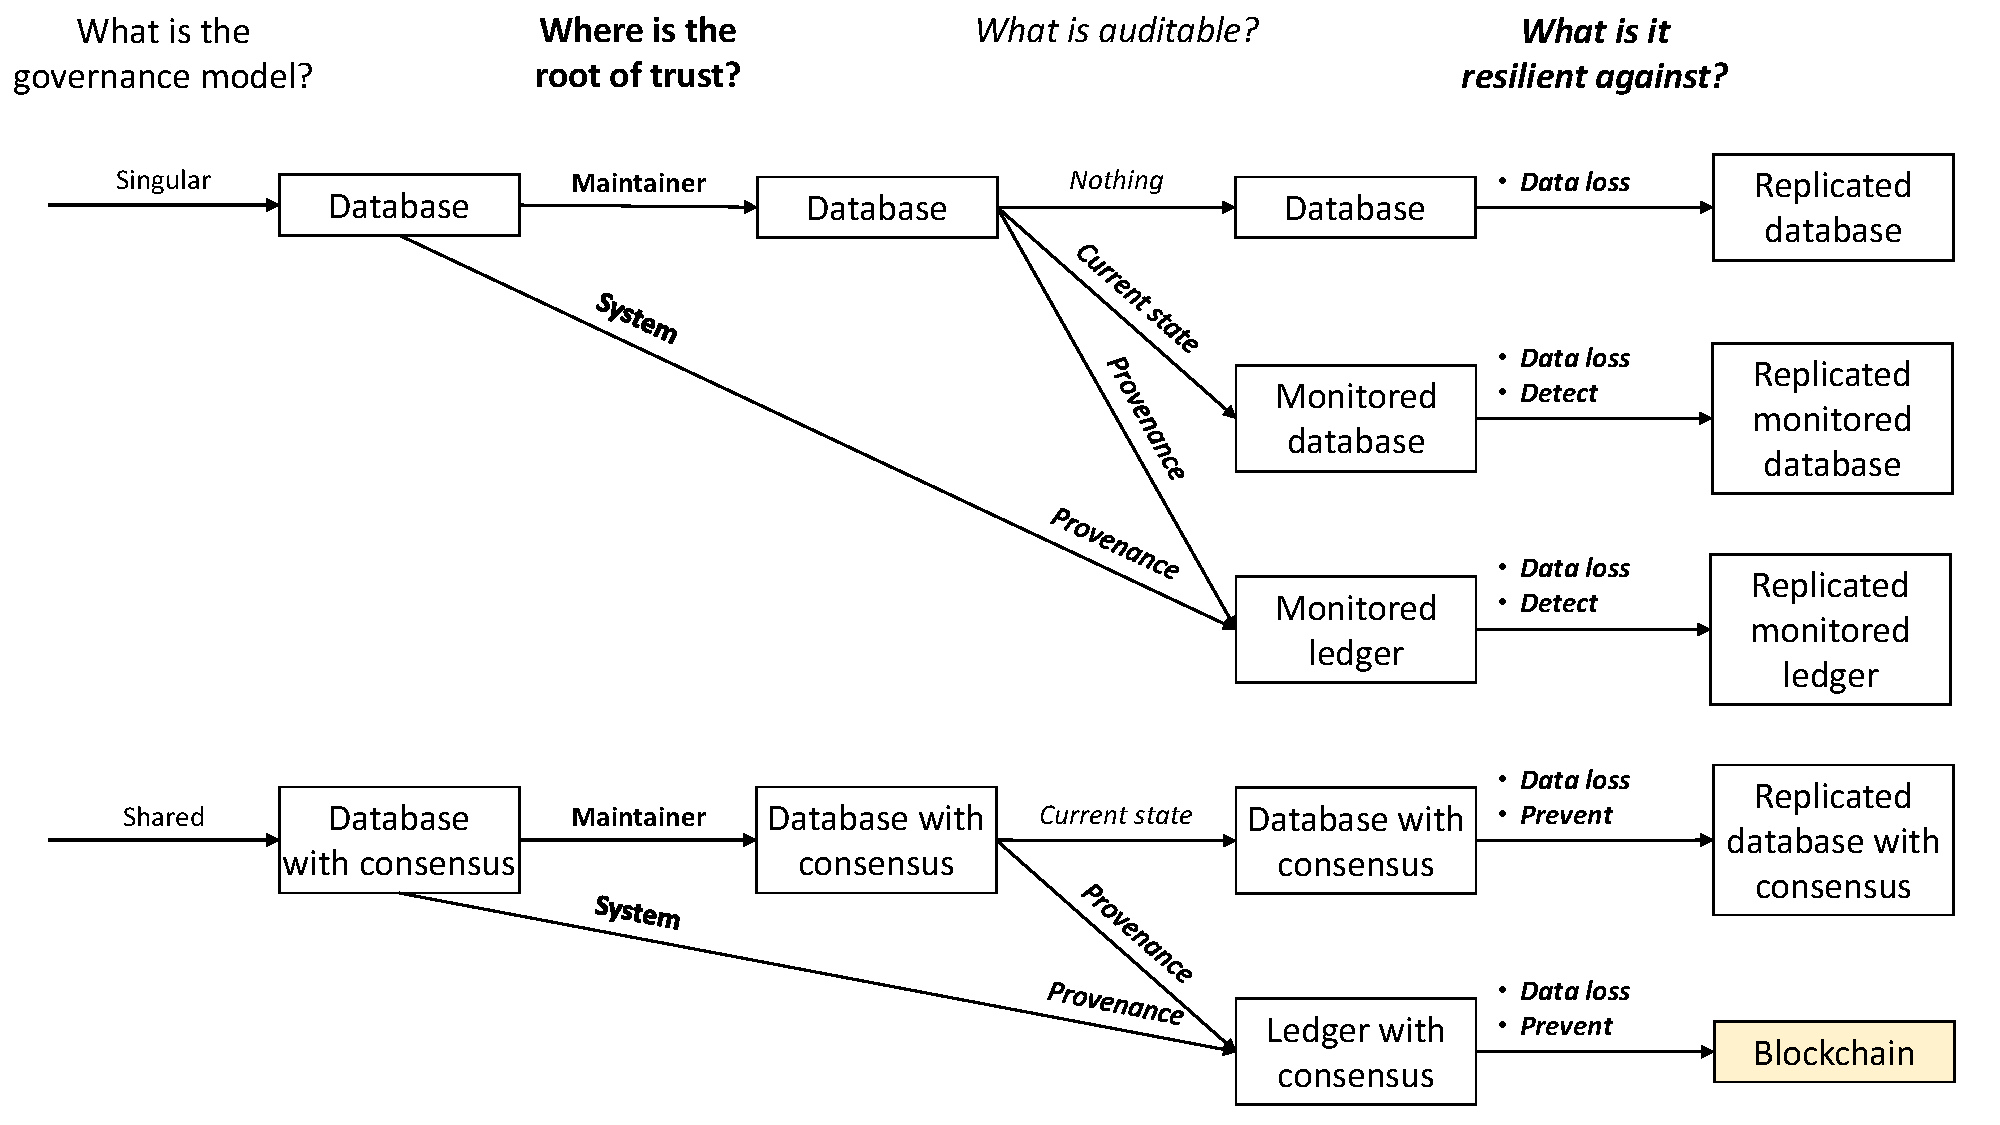
\includegraphics[width=.75\textwidth]{figures/BlockchainFlowchart}
	\caption{Comparing decentralized databases. Blockchain is highlighted in the bottom right corner.}
	\label{fig:blockchainFlowchart}
\end{figure*}

The first property in our taxonomy considers who has the authority to manage and update the database: \emph{what is the governance model?} In a centrally governed database (``Centralized''), a single entity performs these tasks. Alternatively, the system can use a consensus protocol to allow for decentralized governance (``Decentralized'').

Next, we consider the security model by asking \emph{where is the root of trust?}
This refers to the entity or entities that must behave honestly in order for the system to be secure.
In typical database systems, trust is rooted in the maintainer (``Maintainer'')---for example, using AWS cloud storage requires that you trust Amazon.
Alternatively, trust can be rooted in the design of the system itself (``System''), though this is only possible if the system stores sufficient provenance for it to be audited to confirm that the system is functioning as intended.

The next question is \emph{what is auditable?}
In the worst case, nothing is auditable (``Nothing'').
Systems can use an authenticated data structure~\cite{tamassia2003authenticated} to ensure that their current state can be audited (``Current state'').
If the state also contains a history of the system (e.g., a ledger), then the use of an authenticated data structure allows for the provenance of the system to also be audited (``Provenance'').
In both cases, it is necessary that these databases be monitored to ensure that they never enter an invalid state, even temporarily.
In the case of decentralized systems, the decentralized partners can act as monitors.

Finally, we can classify systems by asking \emph{what is it resilient against?}
In particular, we considered with three resiliency properties---(1) is it resilient to accidental data loss (``Data loss''), (2) is it possible to detect that data has been malicious altered (``Detect''), (3) and is it possible to prevent malicious updates (``Prevent'').
Systems with centralized governance are only able to detect malicious updates as the monitors can detect the attack but cannot prevent the malicious update from being replicated.
If we modify the system to allow monitors to play this role, they have become consensus partners and we now have a decentralized database.

% !TEX root = ../main.tex
No content here.


\subsection{Technical Properties Full Diagram}

%\begin{center}
%	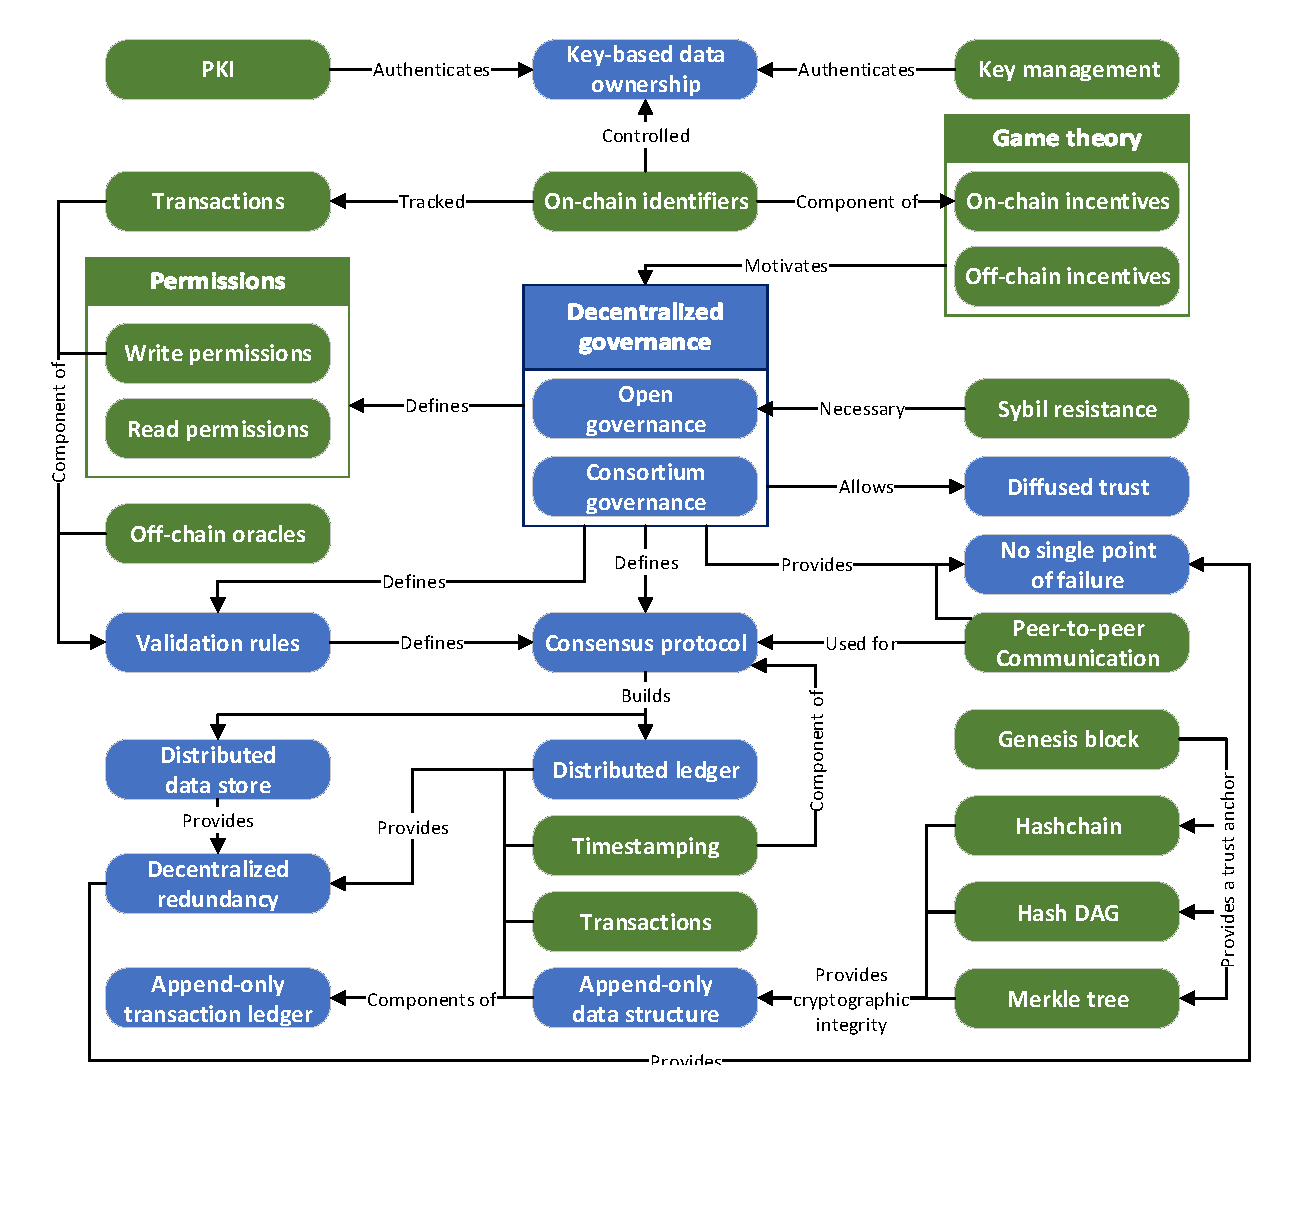
\includegraphics[page=1,width=\columnwidth]{figures/grounded-theory-main}
%	\captionof{figure}{Technical Properties for Blockchain Technology With Supporting Technical Primitives}
%	\label{fig:technical-properties-full}
%\end{center}

\begin{figure}[h]
	\centering
	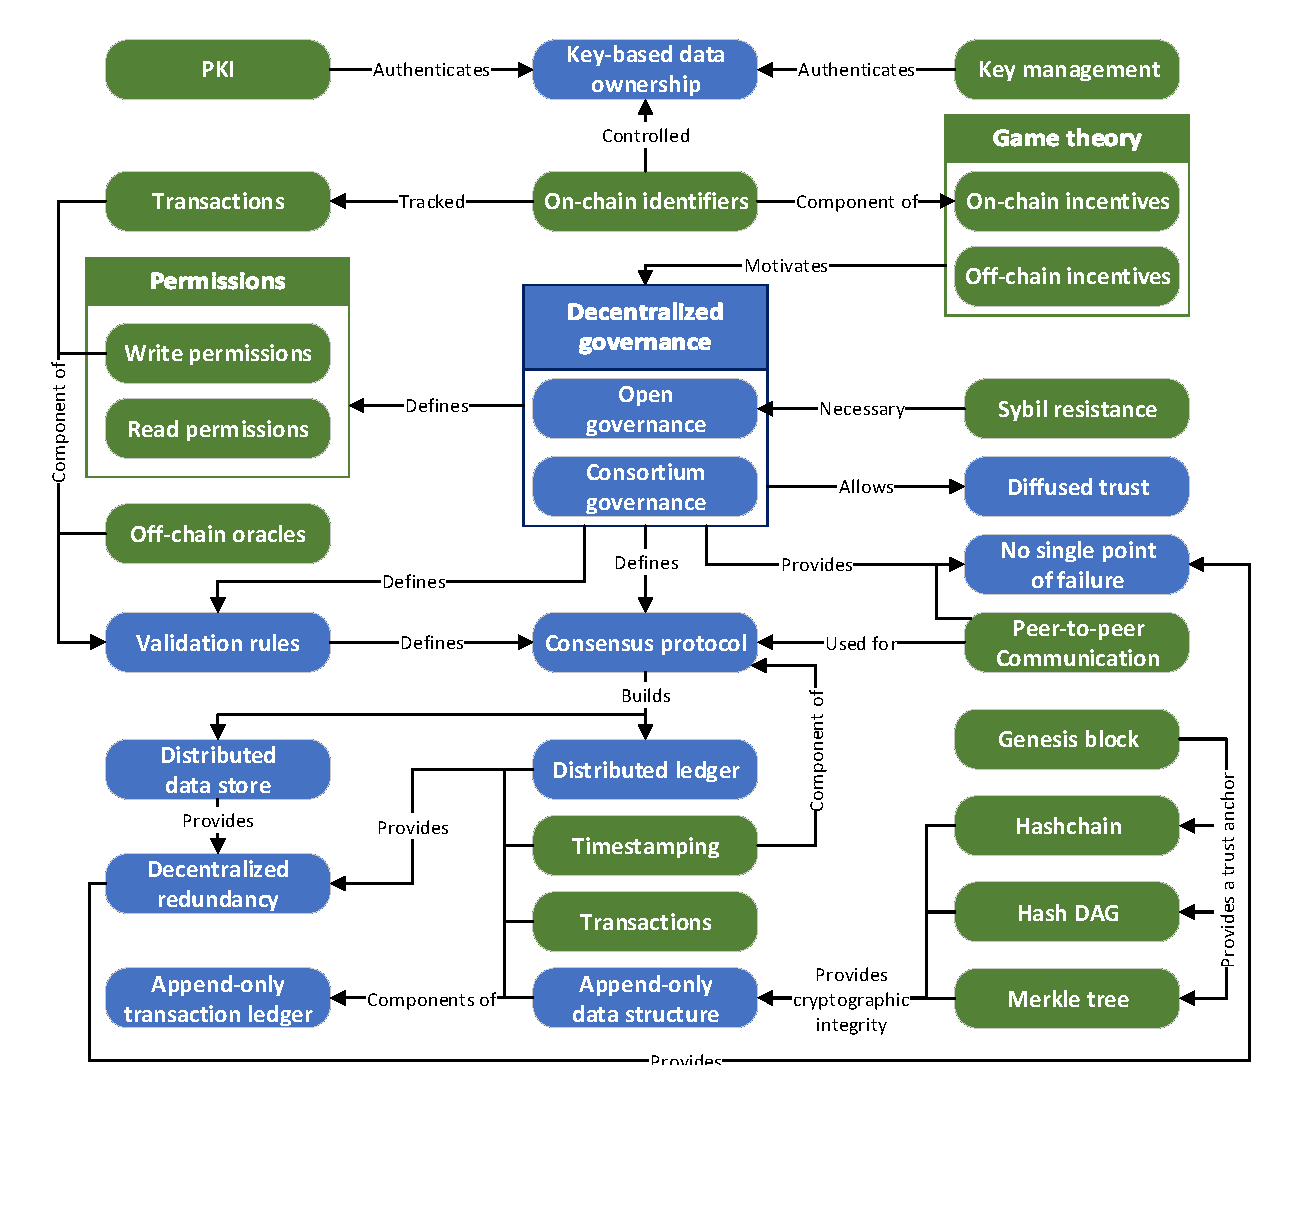
\includegraphics[page=1,width=\columnwidth]{figures/grounded-theory-main}
	
	Technical properties are in blue and technical primitives are in green.
	\caption{Technical Properties for Blockchain Technology With Supporting Technical Primitives}
	\label{fig:technical-properties-full}
\end{figure}